\documentclass{article}
\usepackage[italian]{babel}
\usepackage[T1]{fontenc}
\usepackage{graphicx}
\usepackage[utf8x]{inputenc}
\usepackage{amsmath}
\usepackage{amsthm}
\usepackage{hyperref}
\usepackage{caption}
%\usepackage{tikz}
\date{}
\author{Gruppo 1G.BT \\Lorenzo Cavuoti, Francesco Sacco}
\title{Caratteristiche porte logiche e semplici circuiti logici}

\begin{document}
\maketitle
\paragraph{3)}
	\subparagraph{a)}
		\begin{center}
			\begin{minipage}{.7\linewidth}
				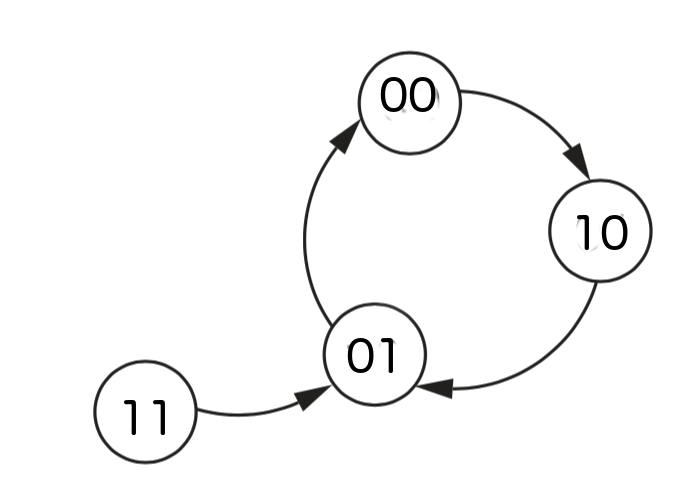
\includegraphics[width=0.5\linewidth]{foto/diagramma_a_stati}
				\captionof{figure}{Diagramma a Stati}
				\label{fig:stati}
			\end{minipage}
		\end{center}
	\subparagraph{b)}
		Indicheremo uno stato $S=Q_1Q_2$ dove $Q_1$ figura \ref{fig:circ} è lo stato del primo flip flop, mentre $Q_2$ è lo stato del secondo flip-flop.\newline
		In totale gli stati sono 3: $00, 01, 10, 11$ lo stato 11 è "in più", nel senso che quando il circuito è a regime gli stati che vengono attivati sono $00,01,10$ come si può vedere in figura\ref{fig:stati}.
	\subparagraph{c)}
		La tabella di verità è la seguente\newline
		\begin{center}
		\begin{tabular}{cc}
			\hline
			$S_n$ & $S_{n+1}$\\
			\hline
			$00$ & $10$\\
			$01$ & $00$\\
			$10$ & $01$\\
			$11$ & $01$\\
			\hline
		\end{tabular}
		\end{center}
	\subparagraph{d)}
		Non essendoci ingressi il circuito è una macchina di Moore (uscite=$f(S_n)$).\newline
		\[
			(Q_1)_{n+1}=\overline{(Q_1)_n+(Q_2)_n}
		\]
		\[
			(Q_2)_{n+1}=(Q_1)_n
		\]
	\subparagraph{e)}
		ma che minchia di domanda è?\footnote{Una risposta del cazzo a una domanda del cazzo}
\end{document}